\section{数据处理与探索性分析}

\subsection{数据来源与格式}

本赛题提供集装箱外表面图像数据集，共 3713 幅图像，其中训练集 3300 幅、测试集 413 幅，图像分辨率统一为 $640\times640$。标注采用 YOLO 标准格式，每个标注框以“类别编号、中心点归一化坐标、宽高归一化值”共五行数据表示。缺陷共三类：Dent（凹陷，编号 0）、Hole（破洞，编号 1）、Rusty（锈蚀，编号 2）。数据集构成如表 \ref{tab:dataset} 所示。

\begin{table}[H]
\centering
\zihao{5}
\caption{数据集构成}\label{tab:dataset}
\begin{tabular}{lcc}
  \toprule
  集合 & 图像数 & 标注框数 \\
  \midrule
  训练集 & 3300 & 8038 \\
  测试集 & 413 & 1066 \\
  \midrule
  合计 & 3713 & 9104 \\
  \bottomrule
\end{tabular}
\end{table}

\subsection{数据集统计特征}

\subsubsection{类别分布}

训练集各类别标注框数量及占比如表 \ref{tab:class_dist} 与图 \ref{fig:class_dist} 所示。可以看出，Dent 类占 48.9\%，Rusty 类占 39.3\%，而 Hole 类仅占 11.8\%，约为 Dent 类的四分之一，类别不平衡问题突出，少数类 Hole 的检测性能需要重点保障。

\begin{table}[H]
\centering
\zihao{5}
\caption{训练集类别分布}\label{tab:class_dist}
\begin{tabular}{lcc}
  \toprule
  类别 & 标注框数 & 占比 \\
  \midrule
  Dent（凹陷） & 3934 & 48.9\% \\
  Hole（破洞） & 946 & 11.8\% \\
  Rusty（锈蚀） & 3158 & 39.3\% \\
  \midrule
  合计 & 8038 & 100.0\% \\
  \bottomrule
\end{tabular}
\end{table}

\begin{figure}[H]
\centering
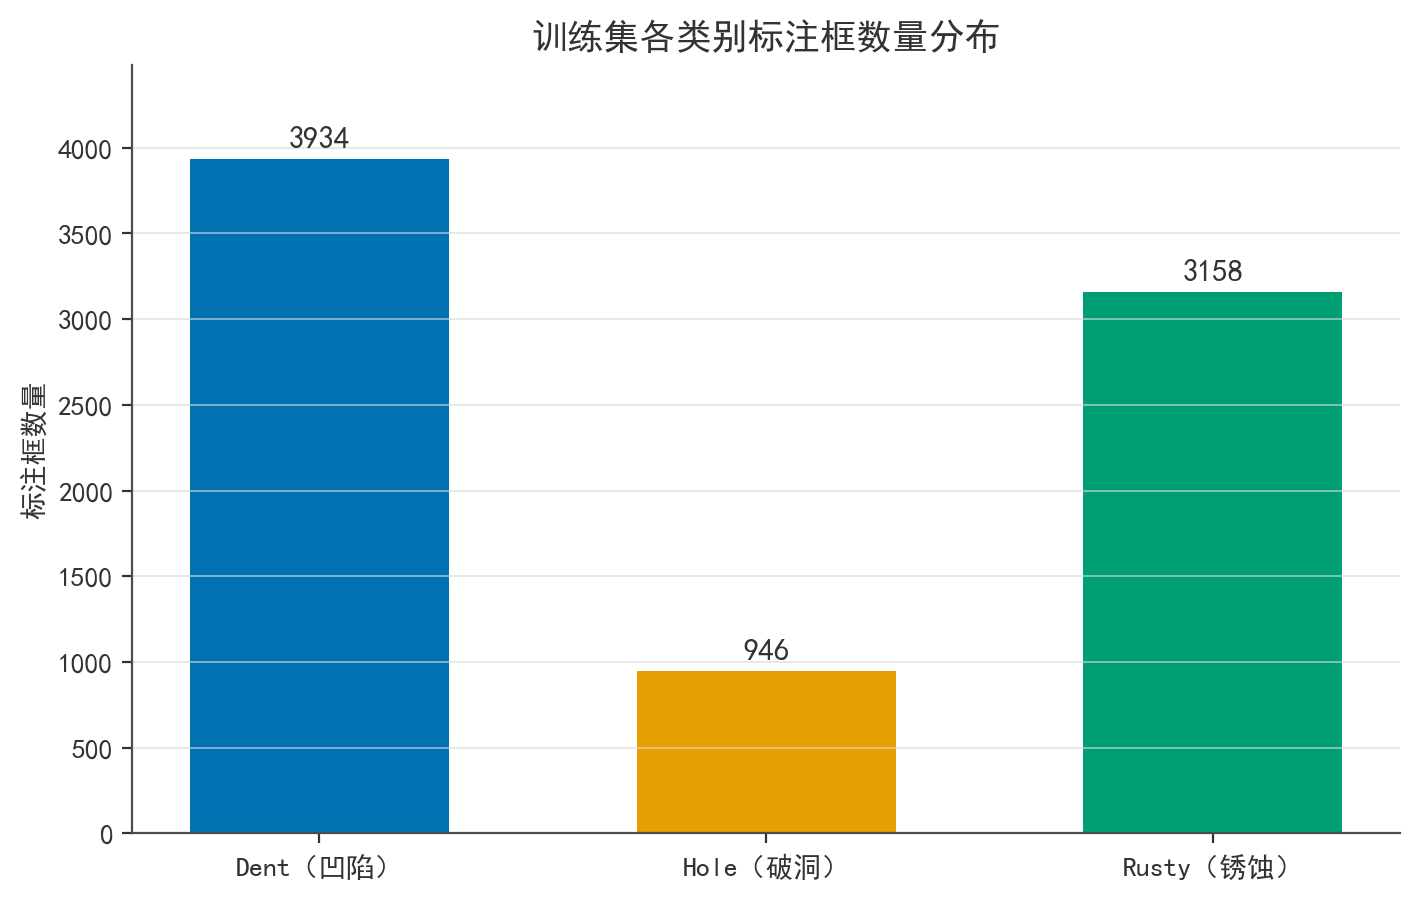
\includegraphics[width=0.62\textwidth]{figures/fig_class_dist.png}
\caption{训练集各类别标注框数量分布}\label{fig:class_dist}
\end{figure}

\subsubsection{每图缺陷数量分布}

训练集每幅图像包含 $1\sim50$ 个缺陷标注，平均每图 2.44 个、中位数 2 个、标准差 2.82。其中含单个缺陷的图像 1619 幅（49.1\%），含多个缺陷的图像 1681 幅（50.9\%），密集目标检测场景占比高，对模型的去重与关联能力提出要求。分布如图 \ref{fig:boxes_per_image} 所示。

\begin{figure}[H]
\centering
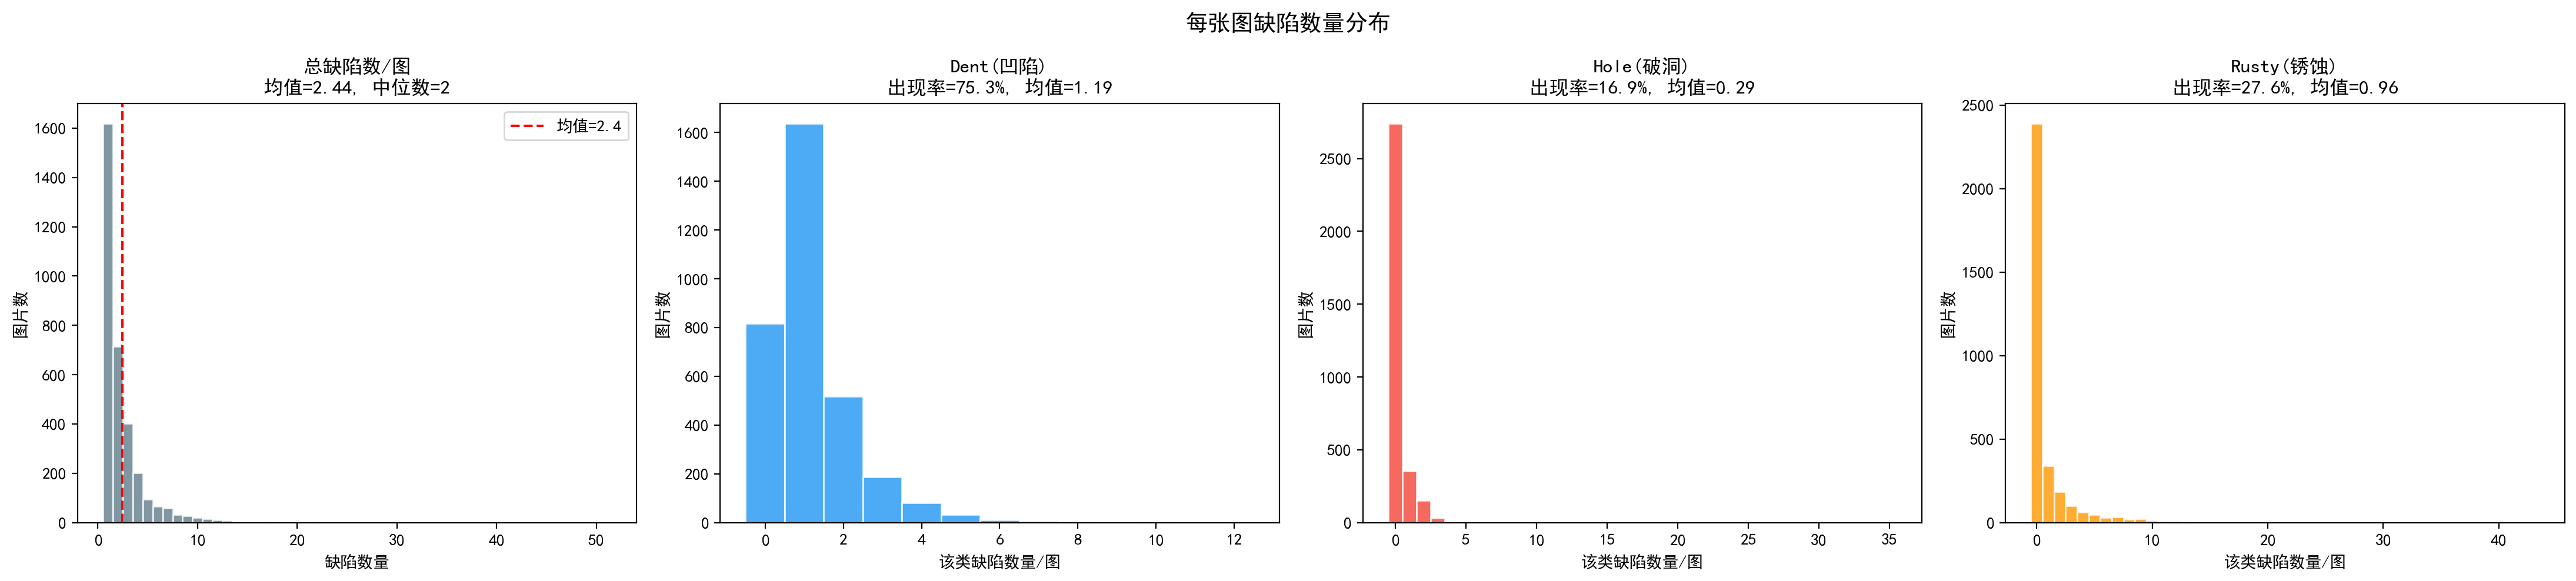
\includegraphics[width=0.75\textwidth]{figures/fig_boxes_per_image.png}
\caption{训练集每图缺陷数量分布}\label{fig:boxes_per_image}
\end{figure}

\subsubsection{目标尺度分布}

按 COCO 标准\cite{lin2014coco}（以 $640\times640$ 为基准，面积小于 $32\times32$ 像素为小目标，$32\times32$ 至 $96\times96$ 为中目标，其余为大目标）统计各尺度占比，结果如表 \ref{tab:scale} 与图 \ref{fig:scale} 所示。全部目标中小目标占比 17.0\%，其中 Hole 类小目标占比高达 43.7\%，尺度差异显著，要求模型具备强多尺度特征提取能力。

\begin{table}[H]
\centering
\zihao{5}
\caption{训练集目标尺度分布（COCO 标准）}\label{tab:scale}
\begin{tabular}{lccc}
  \toprule
  类别 & 小目标 & 中目标 & 大目标 \\
  \midrule
  Dent & 253（6.4\%） & 1487（37.8\%） & 2194（55.8\%） \\
  Hole & 413（43.7\%） & 327（34.6\%） & 206（21.8\%） \\
  Rusty & 700（22.2\%） & 1820（57.6\%） & 638（20.2\%） \\
  \midrule
  全部 & 1366（17.0\%） & 3634（45.2\%） & 3038（37.8\%） \\
  \bottomrule
\end{tabular}
\end{table}

\begin{figure}[H]
\centering
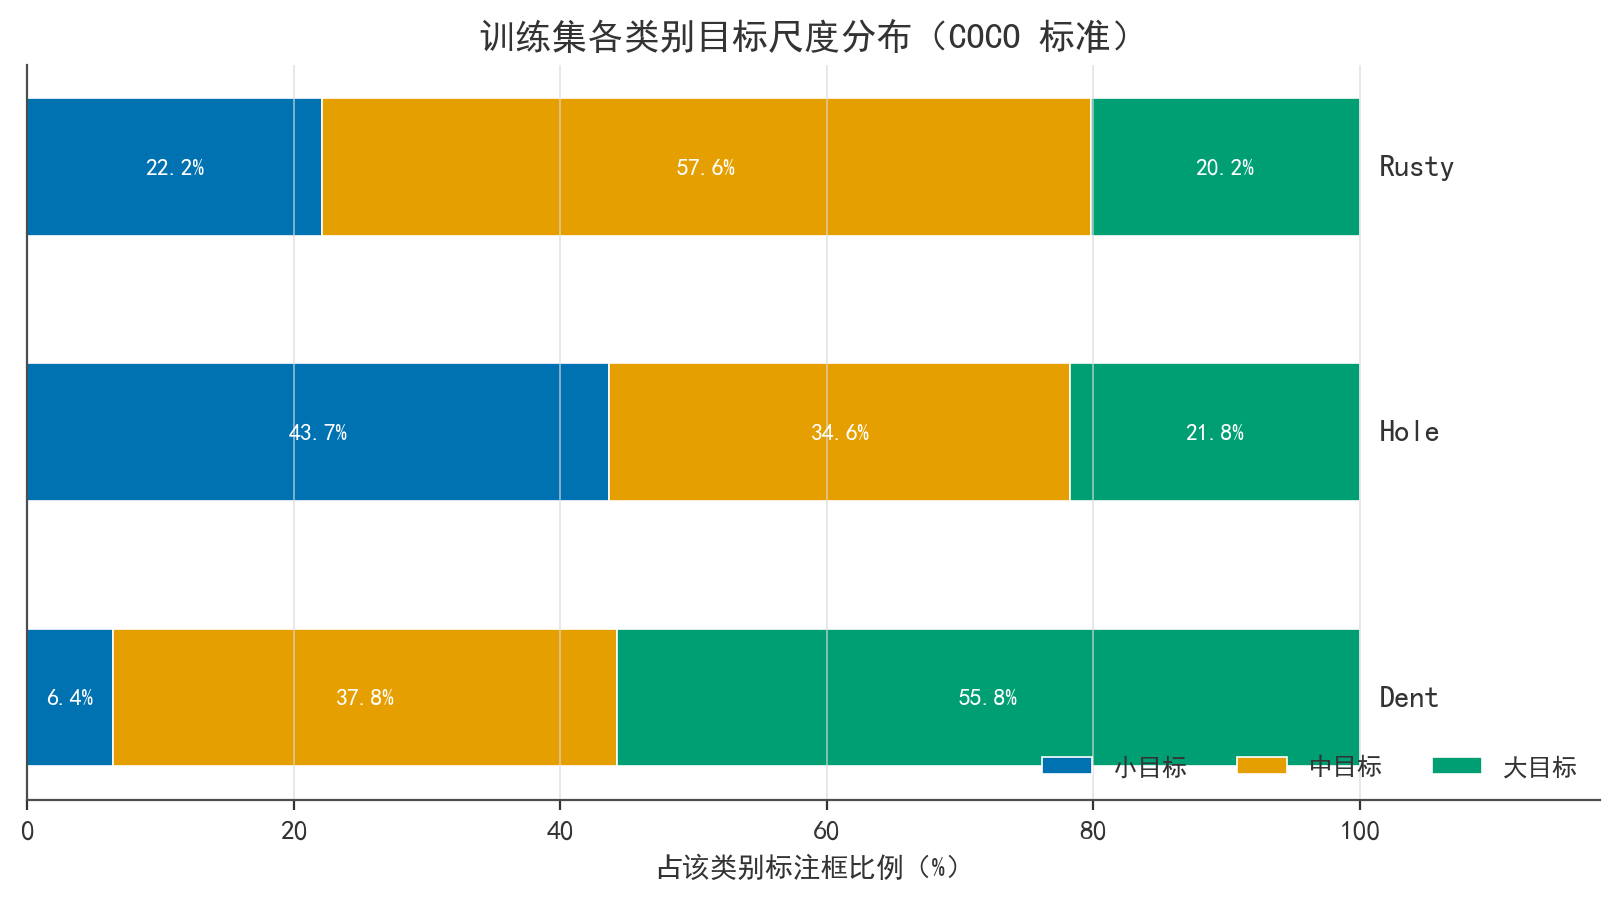
\includegraphics[width=0.72\textwidth]{figures/fig_scale_dist.png}
\caption{训练集目标尺度分布}\label{fig:scale}
\end{figure}

\subsubsection{图像视觉特征}

对训练集图像的亮度、对比度、饱和度与色调进行统计，结果如表 \ref{tab:quality} 与图 \ref{fig:quality} 所示。图像亮度均值 129.5、标准差 41.9，跨度从 13 到 236，光照条件差异极大；对比度与饱和度同样呈现大范围波动。这一特征决定了模型训练必须引入强光照扰动类增强，以覆盖拍摄环境变化。

\begin{table}[H]
\centering
\zihao{5}
\caption{图像视觉特征统计}\label{tab:quality}
\begin{tabular}{lcc}
  \toprule
  统计量 & 均值$\pm$标准差 & 范围 \\
  \midrule
  亮度 & 129.5$\pm$41.9 & $[13,\ 236]$ \\
  对比度 & 49.9$\pm$20.5 & $[8,\ 112]$ \\
  饱和度 & 80.8$\pm$41.6 & $[11,\ 250]$ \\
  色调 & 77.7$\pm$37.9 & $[2,\ 173]$ \\
  \bottomrule
\end{tabular}
\end{table}

\begin{figure}[H]
\centering
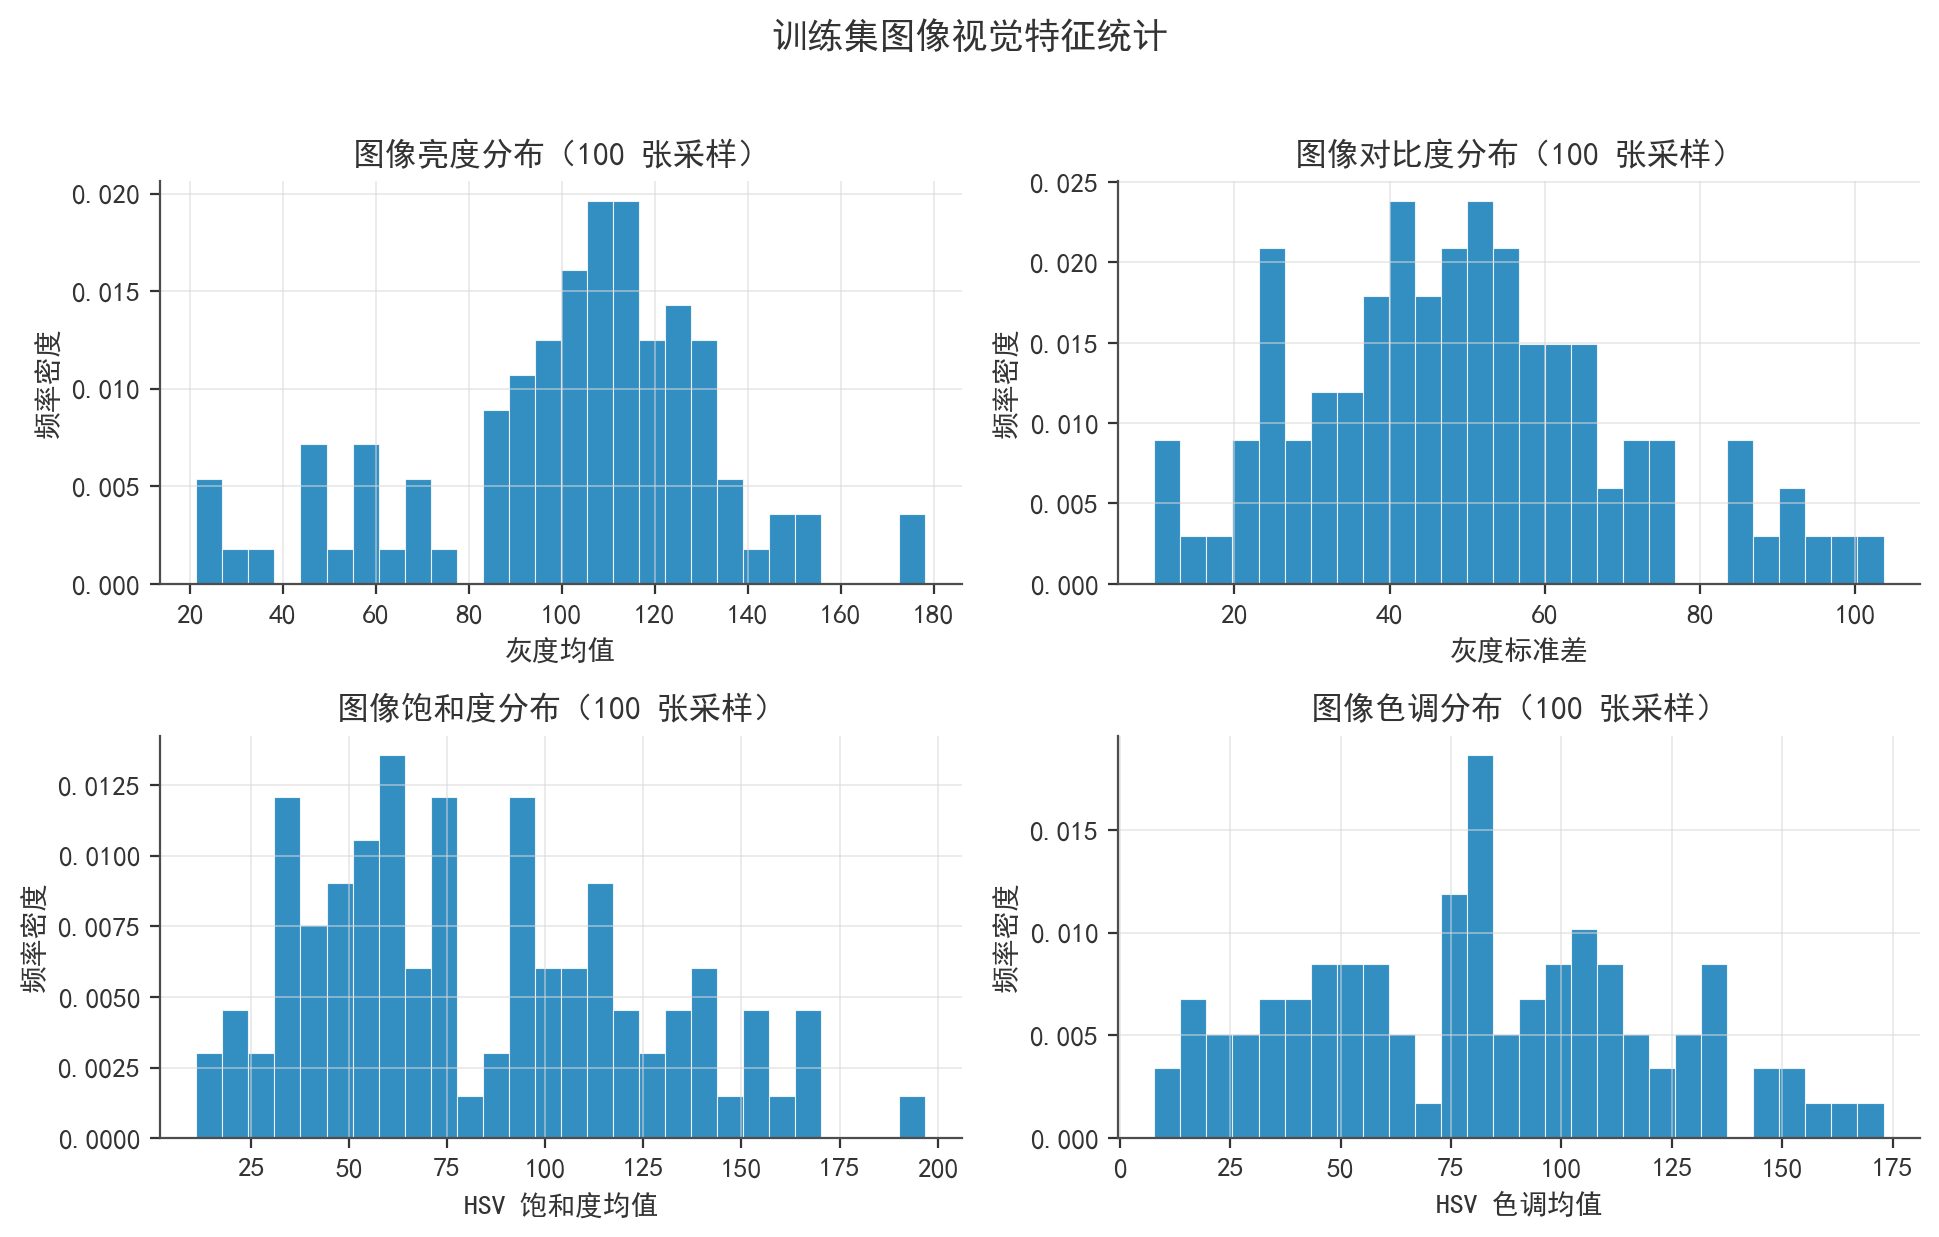
\includegraphics[width=0.9\textwidth]{figures/fig_quality.png}
\caption{图像亮度、对比度与色彩分布}\label{fig:quality}
\end{figure}

此外，标注框位置热力图（图 \ref{fig:heatmap}）显示缺陷在图像空间中的分布相对均匀、无明显区域偏置，但中心区域略密，符合集装箱箱体居中拍摄的成像规律。图 \ref{fig:defect_classes} 给出三类缺陷的典型样本及其标注框示例。

\begin{figure}[H]
\centering
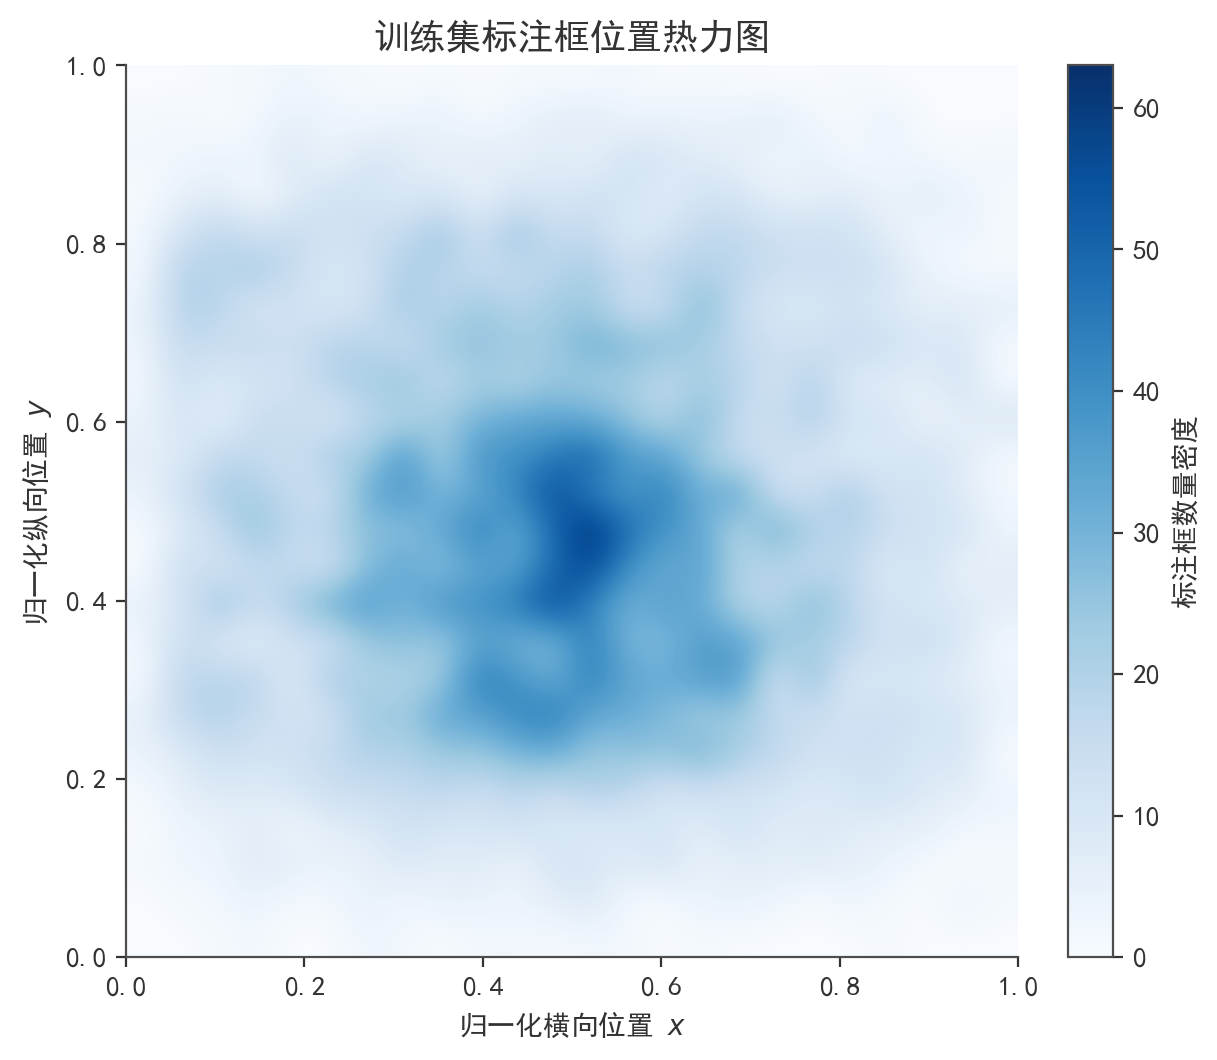
\includegraphics[width=0.6\textwidth]{figures/fig_heatmap.png}
\caption{训练集标注框位置热力图}\label{fig:heatmap}
\end{figure}

\begin{figure}[H]
\centering
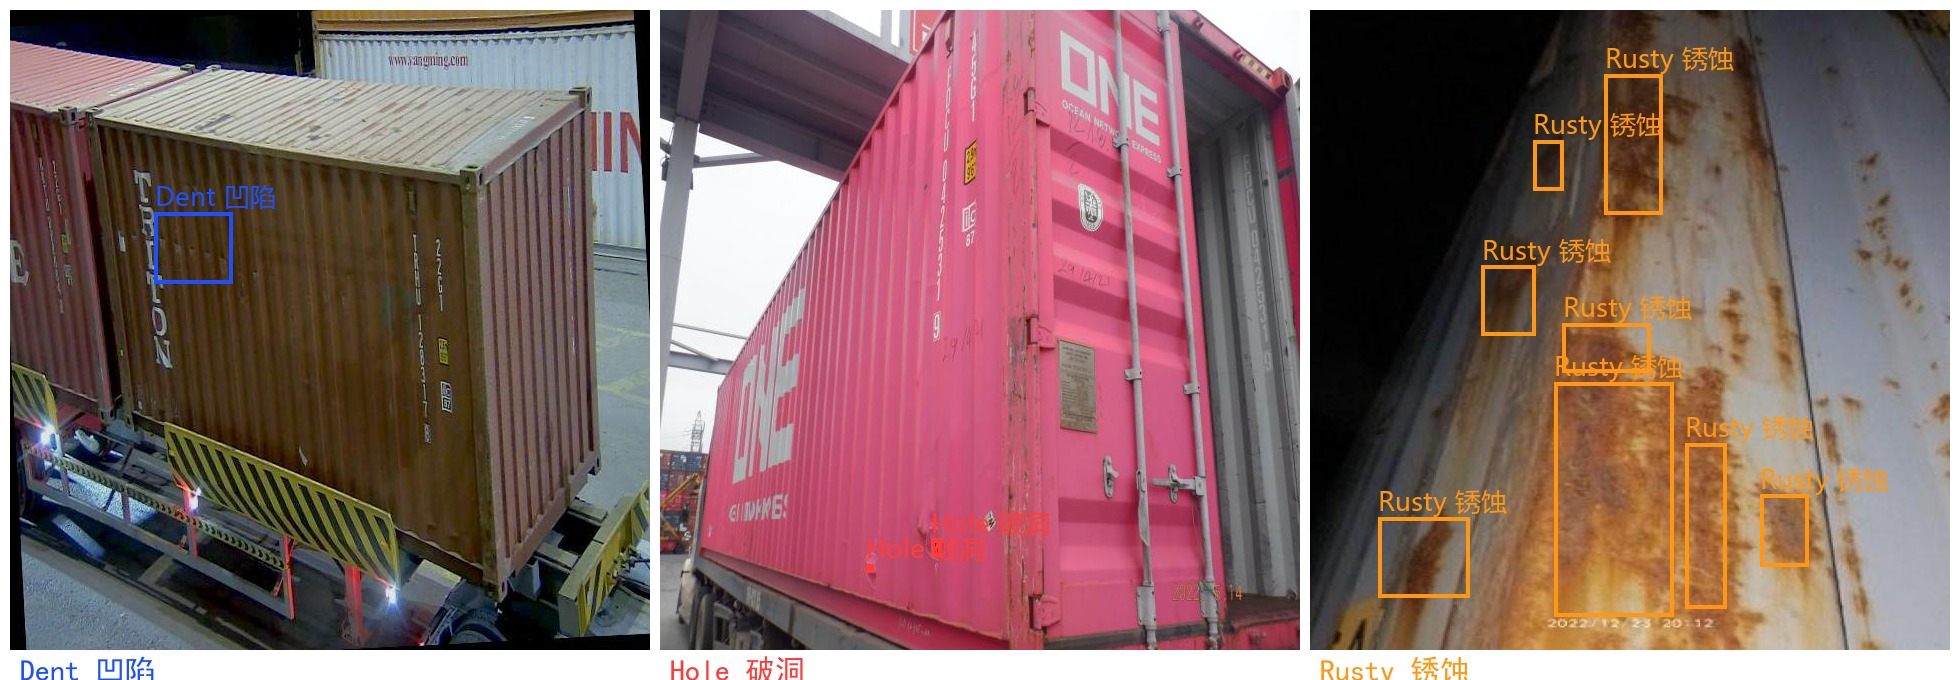
\includegraphics[width=0.95\textwidth]{figures/fig_defect_classes.jpg}
\caption{三类缺陷典型样本（矩形框为数据集标注）}\label{fig:defect_classes}
\end{figure}

\subsection{数据预处理与负样本构造}

针对上述数据特征，本文按以下流程进行数据预处理：

\begin{enumerate}[leftmargin=2.2em,itemsep=2pt]
  \item {\heiti 数据集划分：}按图像主类别进行分层随机抽样，将训练集划分为训练子集 2806 幅与验证子集 494 幅，验证集用于早停与超参数选择；
  \item {\heiti 负样本构造：}训练集不含无缺陷图像，为保证问题一判别模型与检测模型的背景抑制能力，从训练图像中随机选取不覆盖任何标注框的 $320\times320$ 区域进行裁剪，构造候选负样本 1200 幅，其中 600 幅纳入训练集参与检测模型训练（负样本标注文件为空），其余保留备用；
  \item {\heiti 数据增强：}采用表 \ref{tab:aug} 所列的在线增强策略，模拟光照变化、阴影污渍、尺度变化等干扰，提升模型泛化能力。
\end{enumerate}

构造的负样本示例与数据增强效果预览分别见图 \ref{fig:neg_samples} 与图 \ref{fig:aug_preview}。

\begin{table}[H]
\centering
\zihao{5}
\caption{数据增强策略}\label{tab:aug}
\begin{tabular}{lll}
  \toprule
  增强方式 & 参数设置 & 模拟干扰 \\
  \midrule
  HSV 色相/饱和度/亮度扰动 & hsv\_h=0.015, hsv\_s=0.7, hsv\_v=0.4 & 光照变化、反光 \\
  水平翻转 & fliplr=0.5 & 拍摄视角变化 \\
  随机平移与缩放 & translate=0.1, scale=0.5 & 目标尺度变化 \\
  Mosaic 拼接\cite{bochkovskiy2020} & mosaic=1.0 & 复杂背景与遮挡 \\
  Copy-Paste 复制粘贴 & copy\_paste=0.5 & 缓解类别不平衡 \\
  随机擦除 & erasing=0.4 & 阴影、污渍遮挡 \\
  随机增强 & auto\_augment=randaugment & 综合干扰 \\
  \bottomrule
\end{tabular}
\end{table}

\begin{figure}[H]
\centering
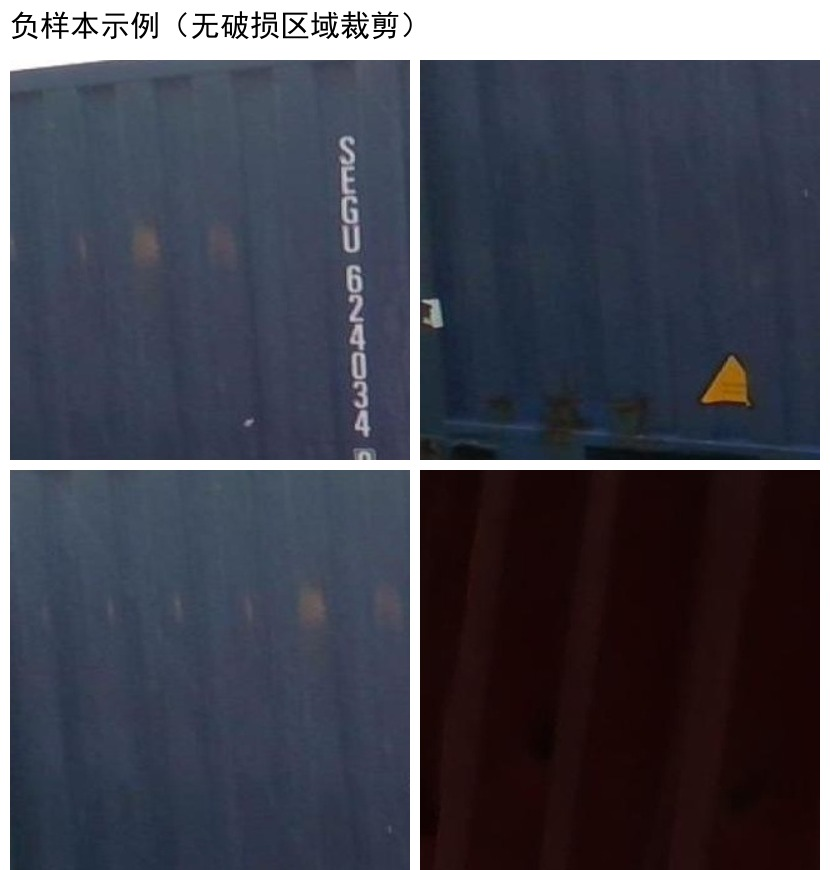
\includegraphics[width=0.92\textwidth]{figures/fig_neg_samples.jpg}
\caption{无标注区域裁剪构造的负样本示例}\label{fig:neg_samples}
\end{figure}

\begin{figure}[H]
\centering
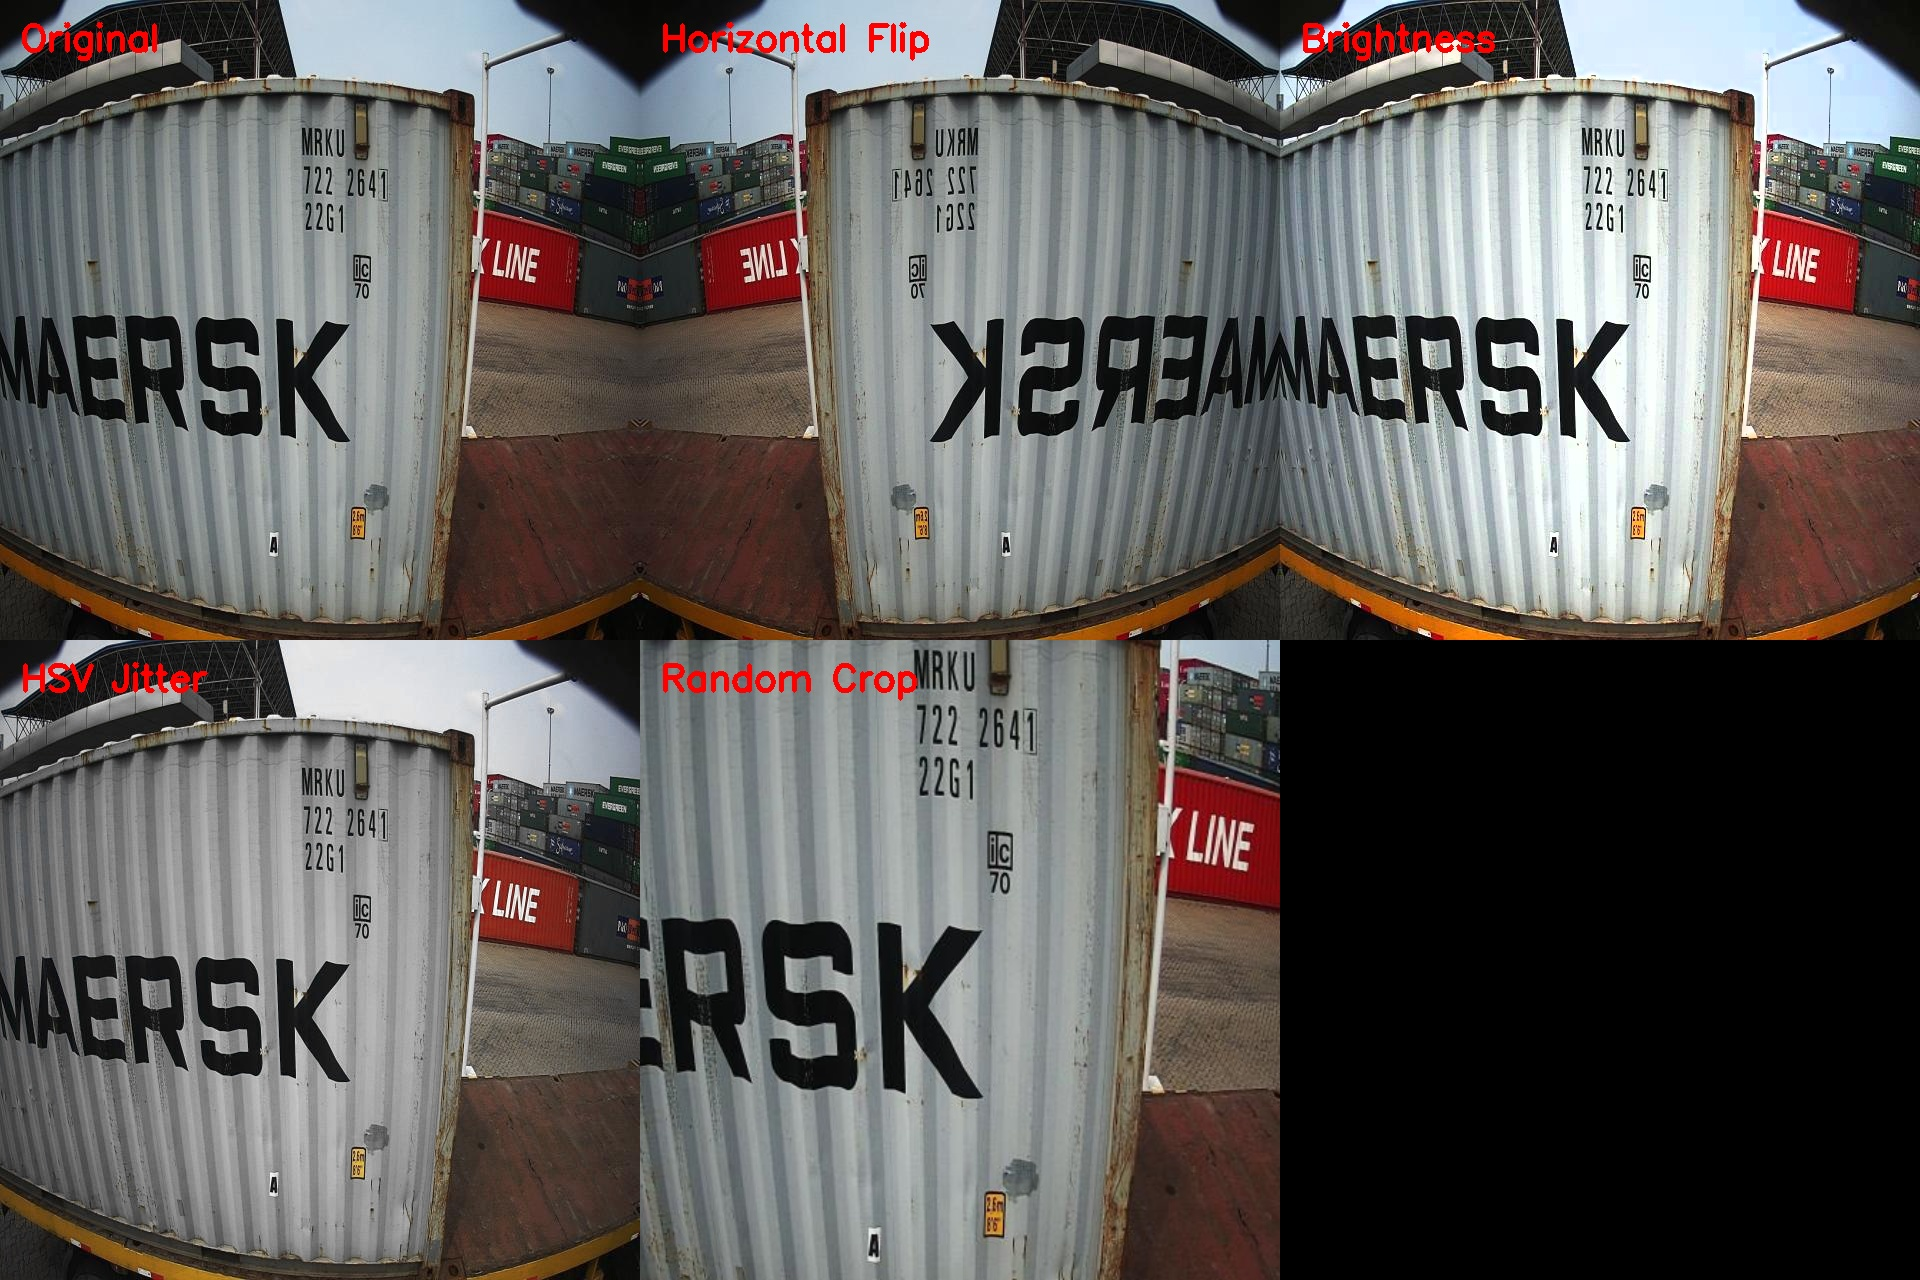
\includegraphics[width=0.95\textwidth]{figures/fig_aug_preview.jpg}
\caption{数据增强效果预览}\label{fig:aug_preview}
\end{figure}

\subsection{小结}

探索性分析表明：本数据集具有类别不平衡（Hole 仅 11.8\%）、小目标占比高（17.0\%）、光照变化剧烈、多目标密集（50.9\% 图像含多个缺陷）且无负样本等特点。上述结论直接指导了后续模型设计与训练策略：采用 Copy-Paste 增强与负样本训练应对不平衡与开放集问题，采用强光照扰动增强应对成像环境差异，采用迁移学习与多尺度检测结构应对小目标与尺度差异。
